%!TeX program = xelatex
\documentclass[12pt,hyperref,a4paper,UTF8]{ctexart}
\usepackage{zjureport}

%%-------------------------------正文开始---------------------------%%
\begin{document}

%%-----------------------封面--------------------%%
\cover

%%------------------摘要-------------%%
\begin{abstract}
本实验致力于构建一个智能家居设备管理系统,能够统一管理和控制多种智能设备,包括灯、空调、窗帘及电视。通过面向对象的设计与实现,本系统满足设备的通用与个性化控制,并通过HomeManager类实现统一的调度与管理。实验通过实际编码和测试,验证了面向对象封装、继承、多态等核心思想在工程开发中的作用。
\end{abstract}

\thispagestyle{empty} % 首页不显示页码

%%--------------------------目录页------------------------%%
\newpage
\tableofcontents

%%------------------------正文页从这里开始-------------------%
\newpage

\section{实验目的和意义}
本实验旨在:
\begin{itemize}
    \item 理解面向对象程序设计思想在实际工程中的应用;
    \item 熟练掌握类的封装、继承、多态及其带来的系统扩展性和维护性优势;
    \item 学会如何统一管理多种智能家居设备,并支持设备个性特性的扩展;
    \item 学会细致分析类的职责与对象关系,为高内聚低耦合的软件设计打下基础。
\end{itemize}

\section{问题描述}
    在实际的智能家居系统中,需要统一管理各类智能设备,对设备开关状态进行控制,并对不同类型设备实现特有控制功能,如调节亮度、温度或打开百分比等,同时需要能够展示所有设备的当前状态。本实验的目标是用面向对象程序设计方式,实现这样一个能够灵活扩展、方便维护和统一控制的智能家居设备管理系统。

\section{需求与实验要求}
\begin{itemize}
    \item 管理多种智能设备,包括智能灯、空调、窗帘等,并可灵活扩展新的设备类型;
    \item 实现设备的统一开关控制接口,并支持各自的特有功能(如亮度调节、温度调节、模式切换等);
    \item 可视化展示所有设备的当前状态(开/关、亮度、温度等);
    \item 支持异常处理,如设备未找到、参数设置非法等情况;
    \item 支持面向对象的场景模式(如“夜间模式”同时控制多设备);
    \item 源代码实现需符合封装、继承、多态、单一职责、开闭原则等面向对象设计原则。
\end{itemize}

\section{实验环境}
\begin{itemize}
    \item 开发工具:VS Code
    \item 编程语言:JavaScript (Node.js)
\end{itemize}

\section{设计思想与实验步骤}
\subsection{总体设计}
设计上,系统采用典型的面向对象分层结构:
\begin{itemize}
    \item 抽象父类 \texttt{SmartDevice} 封装设备共性;
    \item 各设备子类(如 \texttt{SmartLight}、\texttt{SmartAC}、\texttt{SmartCurtain}、\texttt{SmartTV} )分别实现个性化行为;
    \item \texttt{HomeManager} 类负责统一设备管理和调度,体现多态扩展能力;
    \item \texttt{SceneMode} 类体现组合设计思想,实现一组设备的批量自动化控制。
\end{itemize}

\subsection{类结构与继承关系}
见 \autoref{fig:class-diagram}。

\begin{figure}[h!]
    \centering
    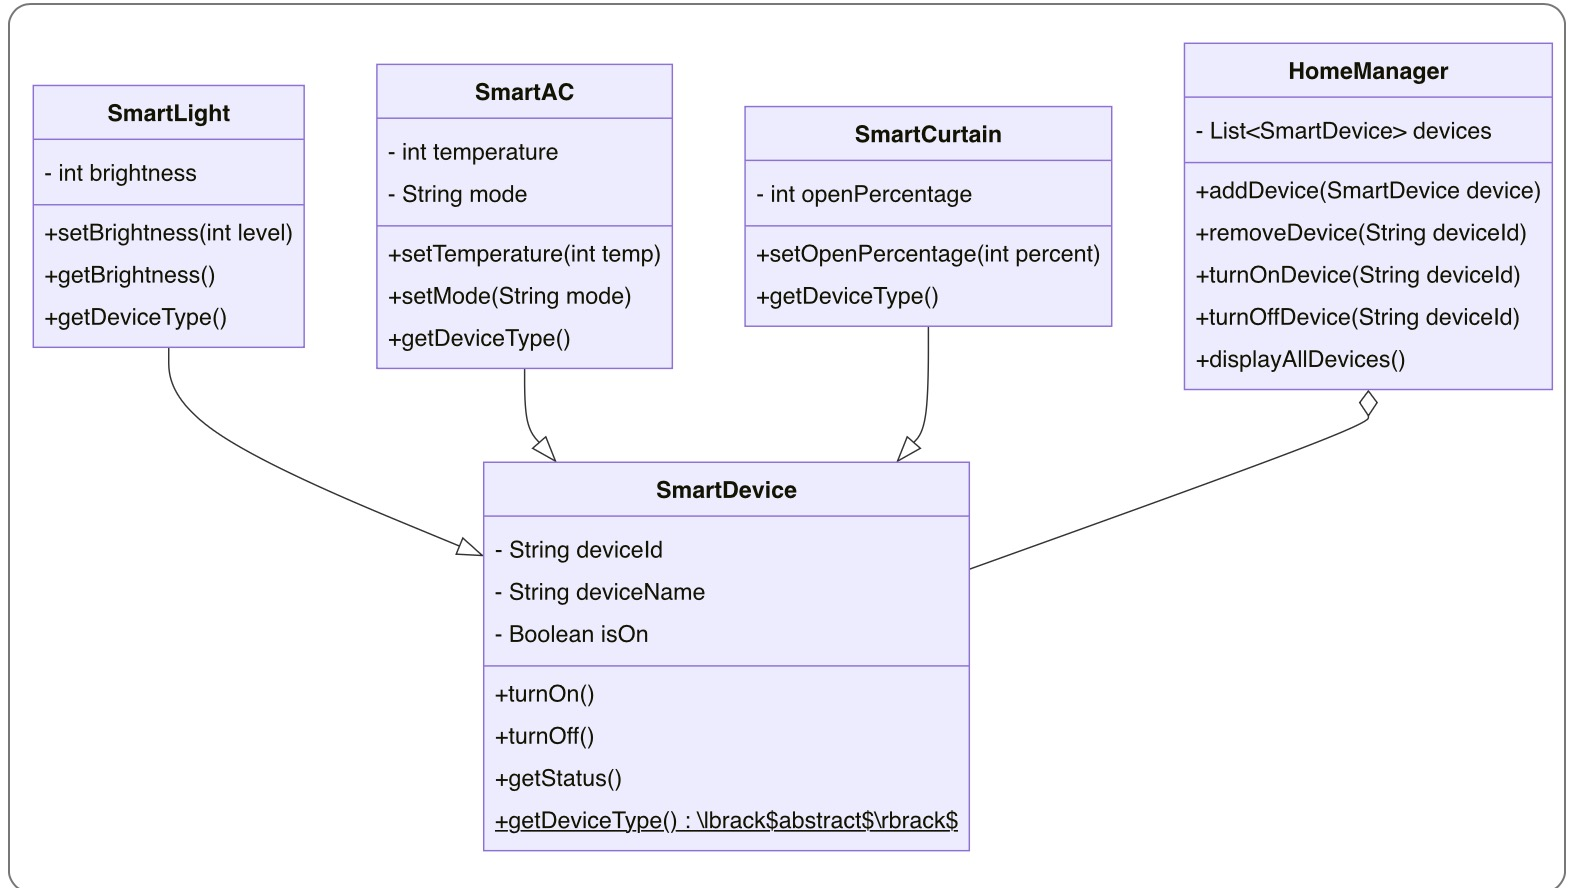
\includegraphics[width=.75\textwidth]{../lab2/class_diagram.png} % 可手动导出mermaid图为图片后放在lab2
    \caption{智能家居系统类图}
    \label{fig:class-diagram}
\end{figure}

\subsection{主要类及方法说明}
\begin{itemize}
    \item \textbf{Controllable(接口)}:定义统一的 \texttt{turnOn}/\texttt{turnOff} 方法(接口/ABC)。
    \item \textbf{SmartDevice(抽象父类)}:所有设备的统一属性和通用方法;ID、名称、开关状态私有化存储,暴露公共只读接口。
    \item \textbf{SmartLight / SmartAC / SmartCurtain / SmartTV(具体设备子类)}:分别实现特有的控制能力,如设置亮度、温度、频道、音量等。
    \item \textbf{HomeManager}:存储和管理全部设备实例,提供加入/移除/统一控制及展示能力。
    \item \textbf{SceneMode}:聚合多个“动作”,实现场景控制模式。
\end{itemize}

\subsection{计算步骤及核心流程}
\begin{enumerate}
    \item 定义统一抽象父类及接口→实现各个具体智能设备→统一加入HomeManager管理。
    \item 通过HomeManager批量控制、展示、异常处理。
    \item 通过SceneMode实现批量场景模式并测试正确性。
\end{enumerate}

\section{主要实现与测试}
\subsection{部分主要源代码}
(完整代码见附录/lab2目录,下方为部分核心片段摘录)

% 代码示例(节选,详见lab2目录)
\begin{verbatim}
// SmartDevice.js
class SmartDevice {
    constructor(deviceId, deviceName) {
        if (new.target === SmartDevice) {
            throw new Error("不能直接实例化SmartDevice抽象类");
        }
        this._deviceId = deviceId;
        this._deviceName = deviceName;
        this._isOn = false;
    }
    turnOn() { this._isOn = true; }
    turnOff() { this._isOn = false; }
    getStatus() { return this._isOn ? "开" : "关"; }
    get deviceId() { return this._deviceId; }
    get deviceName() { return this._deviceName; }
    get isOn() { return this._isOn; }
    getDeviceType() { throw new Error("请在子类中实现getDeviceType方法"); }
}

// SmartLight.js
class SmartLight extends SmartDevice {
    constructor(deviceId, deviceName, brightness = 100) {
        super(deviceId, deviceName);
        this._brightness = brightness;
    }
    setBrightness(level) { /* ... */ }
    getDeviceType() { return "智能灯"; }
    getStatus() { return `${super.getStatus()},亮度:${this._brightness}`; }
}
// ... 其余代码见附件 ...
\end{verbatim}

\subsection{功能与效果展示}
\begin{itemize}
    \item 支持多种类型设备,灵活增减,且能统一开关与特有功能控制;
    \item 支持一次控制多设备场景,如一键夜间模式:\texttt{SceneMode}批量设置行为;
    \item 完善的异常处理与边界条件检验,如ID重复,参数非法等都能给出明确提示。
\end{itemize}

\section{关键问题分析与回答}
\subsection{封装分析}
\textbf{被封装的属性:} 如 \_deviceId、\_deviceName、\_isOn 等全部设为私有(类内访问),通过getter暴露只读访问接口。封装的目的是防止外部直接篡改,增强类的健壮性与安全性,保护对象一致性。

\subsection{继承层次与说明}
见~\autoref{fig:class-diagram}。
各设备子类(灯、空调、窗帘、电视)均继承SmartDevice的共性(ID、名称、开关、状态展示等),并根据不同子类实现额外专有操作(如亮度、温度、模式等)。

\subsection{多态体现}
HomeManager中的设备操作方法(如turnOnDevice、turnOffDevice和displayAllDevices),是通过调用基类接口来操作不同子类对象,具体运行时会自动分发到正确的子类实现(如getStatus、turnOn),这是多态机制的直接体现。

\subsection{类的扩展性与修改性}
如果添加新设备类型,只需新增对应子类,无需更改HomeManager的核心逻辑。因为其对所有设备采用了接口/基类依赖,不需区分具体类型。这符合开闭原则(对扩展开放,对修改封闭)。

\subsection{设计原则分析}
\begin{itemize}
  \item \textbf{开闭原则:} 只需扩展即可接入新设备类型,无需大规模更改已有代码。
  \item \textbf{单一职责:} 每个类职责单一,SmartXxx仅描述单一设备,HomeManager负责管理,SceneMode负责场景。
\end{itemize}

\subsection{改进建议}
\begin{itemize}
    \item 可增加设备与网络/用户的交互、事件推送、远程控制等功能。
    \item 设备属性和方法可进一步抽象为接口,提升灵活性。
    \item 可集成数据库和前端页面,提升可视化及数据持久化能力。
\end{itemize}

\reference


\end{document}